%% research_paper.tex
%% TrustVault: Trustless, Scalable, and Low-Cost On-Chain Academic
%% Credential Verification Using Internet Computer Protocol
%%
%% IEEE Conference Style — compile with pdflatex (or lualatex)
%% Required packages: IEEEtran, tikz, pgfplots, pgfplotstable,
%%                    amsmath, booktabs, hyperref

\documentclass[conference,a4paper]{IEEEtran}

%% ---------- packages ----------
\usepackage[T1]{fontenc}
\usepackage[utf8]{inputenc}
\usepackage{amsmath,amssymb}
\usepackage{graphicx}
\usepackage{booktabs}
\usepackage{array}
\usepackage{multirow}
\usepackage{url}
\usepackage{hyperref}
\hypersetup{colorlinks=false, pdfborder={0 0 0}}

%% TikZ + PGFPlots for all figures
\usepackage{tikz}
\usetikzlibrary{
  arrows.meta, positioning, shapes.geometric,
  shapes.misc, fit, calc,
  decorations.pathreplacing, backgrounds
}
\usepackage{pgfplots}
\pgfplotsset{compat=1.18}
\usepackage{pgfplotstable}

%% listings for small code snippets
\usepackage{listings}
\lstset{
  basicstyle=\ttfamily\scriptsize,
  breaklines=true,
  frame=single,
  captionpos=b
}

%% ---------- custom colours ----------
\definecolor{icpblue}{RGB}{59,130,246}
\definecolor{icpgreen}{RGB}{34,197,94}
\definecolor{icpyellow}{RGB}{234,179,8}
\definecolor{icppurple}{RGB}{139,92,246}
\definecolor{icpred}{RGB}{239,68,68}
\definecolor{icpgray}{RGB}{100,116,139}
\definecolor{lightblue}{RGB}{219,234,254}
\definecolor{lightgreen}{RGB}{220,252,231}
\definecolor{lightyellow}{RGB}{254,249,195}
\definecolor{lightpurple}{RGB}{237,233,254}

% =========================================================
\begin{document}

\title{TrustVault: Trustless, Scalable, and Low-Cost\\On-Chain Academic Credential Verification\\Using Internet Computer Protocol}

\author{
  \IEEEauthorblockN{Dr.\ Shruti Jadon}
  \IEEEauthorblockA{
    Department of Computer Science\\
    PES University\\
    Bengaluru, Karnataka, India\\
    shrutijadon@pes.edu
  }
  \and
  \IEEEauthorblockN{Varun Gudamsetti}
  \IEEEauthorblockA{
    Department of Computer Science\\
    PES University\\
    Bengaluru, Karnataka, India\\
    varun.techmail@gmail.com
  }
  
}

\maketitle

% =========================================================
\begin{abstract}
Academic credential fraud imposes significant costs on institutions and employers worldwide. Existing solutions rely on either centralized registries or permissioned blockchains, both of which retain trust dependencies and single points of failure. This paper presents \textit{TrustVault}, a fully on-chain academic credential verification system implemented and evaluated on the Internet Computer Protocol (ICP) mainnet. TrustVault stores both credential data and the verification frontend inside ICP canisters and uses ICP \textit{Certified Variables} — backed by threshold BLS signatures from a decentralized subnet — for mathematically verifiable, zero-trust credential verification. An incremental binary Merkle tree provides O($\log n$) update cost as the credential database scales, with each leaf representing a cryptographic commitment to a certificate record. Mainnet benchmarks conducted in March 2026 recorded issuance latency of $\approx$1.9\,s, verification queries as fast as 60\,ms, parallel throughput up to 7.3\,certs/s, concurrent mixed-load throughput of 13.1\,ops/s, and issuance cost of $\approx$\$0.00002 per certificate — over 10{,}000$\times$ cheaper than comparable Ethereum operations. The prototype demonstrates practical feasibility; production deployment requires cryptographic hash hardening.
\end{abstract}

\begin{IEEEkeywords}
Internet Computer Protocol, Academic Credential Verification, Certified Variables, Merkle Tree, Zero-Trust, Motoko, Threshold BLS Signatures
\end{IEEEkeywords}

% =========================================================
\section{Introduction}
\label{sec:intro}

Academic credential fraud is a well-documented, escalating problem: studies estimate that a significant fraction of professional job applications misrepresent qualifications \cite{chahal2021credential}, and traditional verification — contacting institutions manually — is slow, expensive, and centralized. Blockchain-based alternatives have been proposed but each carries practical limitations. Bitcoin and Ethereum anchor credential hashes at prohibitive gas fees (tens of dollars per write), and the verification UI remains on a central server. Permissioned ledgers such as Hyperledger Fabric reduce cost but reintroduce consortium trust \cite{androulaki2018fabric}. Hybrid systems storing only hashes on-chain with data off-chain restore centralization through the back door.

The \textit{Internet Computer Protocol} (ICP) \cite{hanke2018dfinity} offers a qualitatively different model. ICP runs smart contracts called \textit{canisters} — WebAssembly modules replicated across independent \textit{subnets} of geographically diverse nodes. Consensus achieves finality in $\approx$1--3\,s via a BFT notarization protocol backed by the \textit{Random Beacon} (threshold BLS over previous round outputs). Two protocol features are critical to this work: \textit{on-chain web serving} (canisters respond to HTTP, eliminating cloud hosting) and \textit{Certified Variables} (a native API where a canister commits a 32-byte value that the subnet collectively signs with a threshold BLS key \cite{dfinity2022geeks}, enabling data verification with no trust in the canister or any single node). Query calls — read-only operations bypassing consensus — return in $<$500\,ms at no cost to the caller.

\textbf{Contributions:}
\begin{itemize}
  \item TrustVault — among the first fully on-chain academic credential systems (frontend \emph{and} backend) deployed and evaluated on a public blockchain mainnet, with reproducible real-world measurements.
  \item An incremental Merkle tree with O($\log n$) update cost, integrated with Certified Variables for trustless proof generation.
  \item A rigorous mainnet evaluation conducted in March 2026: issuance, verification, throughput, finality, and concurrent mixed-load.
  \item A cross-platform comparison against Ethereum PoS \cite{buterin2020eth2} and Hyperledger Fabric \cite{androulaki2018fabric} using only published benchmarks.
\end{itemize}

% =========================================================
\section{System Design}
\label{sec:design}

\subsection{Architecture}
The Motoko backend is organized into five modules: \textbf{main.mo} (public actor — \texttt{issueCertificate}, \texttt{revokeCertificate}, \texttt{verifyCertificate}), \textbf{CertificateManager.mo} (record hashing and management), \textbf{MerkleTree.mo} (incremental binary Merkle tree), \textbf{Utils.mo} (hex encoding, hash combination), and \textbf{PerformanceMetrics.mo} (telemetry). The frontend is a React + Vite single-page application inside an ICP asset canister, served directly over HTTPS from the blockchain with no external hosting. It communicates with the backend through auto-generated Candid type bindings. Fig.~\ref{fig:sysarch} illustrates the full system.

\begin{figure}[t]
\centering
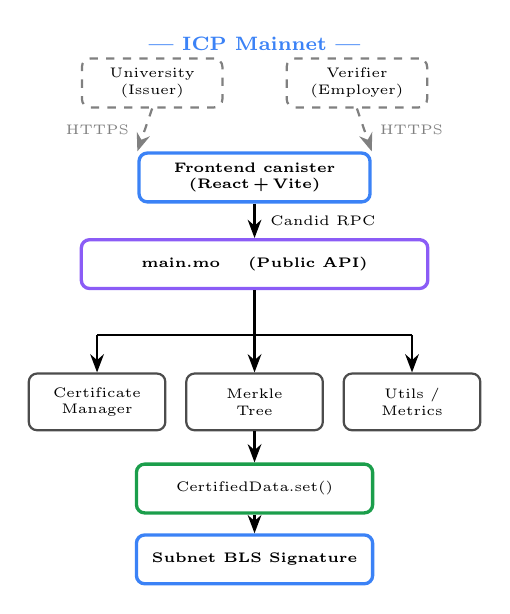
\begin{tikzpicture}[
  actor/.style={rectangle, rounded corners=3pt, draw=gray, dashed, thick,
                minimum height=0.62cm, minimum width=1.65cm, text width=1.55cm,
                font=\tiny, align=center},
  fe/.style={rectangle, rounded corners=3pt, draw=icpblue, very thick,
             minimum height=0.62cm, minimum width=2.8cm, text width=2.7cm,
             font=\tiny\bfseries, align=center},
  api/.style={rectangle, rounded corners=3pt, draw=icppurple, very thick,
              minimum height=0.62cm, minimum width=4.4cm,
              font=\tiny\bfseries, align=center},
  mod/.style={rectangle, rounded corners=3pt, draw=black!70, thick,
              minimum height=0.72cm, minimum width=1.6cm, text width=1.5cm,
              font=\tiny, align=center},
  certd/.style={rectangle, rounded corners=3pt, draw=icpgreen!80!black, very thick,
                minimum height=0.62cm, minimum width=3.0cm,
                font=\tiny, align=center},
  bls/.style={rectangle, rounded corners=3pt, draw=icpblue, very thick,
              minimum height=0.62cm, minimum width=3.0cm,
              font=\tiny\bfseries, align=center},
  arr/.style={-Stealth, thick},
  every node/.style={font=\tiny}
]
  %% Sub-modules: centers at x=0, 2.0, 4.0 (gap = 0.4cm between each box)
  \node[mod] (cm) at (0.0, 0.0) {Certificate\\Manager};
  \node[mod] (mt) at (2.0, 0.0) {Merkle\\Tree};
  \node[mod] (ut) at (4.0, 0.0) {Utils /\\Metrics};

  %% main.mo centered at x=2.0
  \node[api] (main) at (2.0, 1.75) {\textbf{main.mo} \quad (Public API)};

  %% Frontend centered at x=2.0
  \node[fe] (front) at (2.0, 2.85) {Frontend canister (React\,+\,Vite)};

  %% External actors symmetric about x=2.0
  \node[actor] (uni) at (0.7, 4.05) {University\\(Issuer)};
  \node[actor] (ver) at (3.3, 4.05) {Verifier\\(Employer)};

  %% ICP Mainnet label (text only)
  \node[font=\scriptsize\bfseries, icpblue] at (2.0, 4.55)
    {--- ICP Mainnet ---};

  %% CertifiedData and Subnet BLS below MerkleTree
  \node[certd] (cd)  at (2.0, -1.10) {CertifiedData.set()};
  \node[bls]   (sub) at (2.0, -2.00) {Subnet BLS Signature};

  %% Actors → Frontend (nearly straight vertical, just slightly inward)
  \draw[arr, dashed, gray] (uni.south) --
    node[left=2pt, font=\tiny, pos=0.5]{HTTPS} (front.north west);
  \draw[arr, dashed, gray] (ver.south) --
    node[right=2pt, font=\tiny, pos=0.5]{HTTPS} (front.north east);

  %% Frontend → main.mo
  \draw[arr] (front.south) --
    node[right=2pt, font=\tiny]{Candid RPC} (main.north);

  %% main.mo → sub-modules via horizontal bus (no diagonal crossing)
  \draw[thick] (main.south) -- (2.0, 0.85);      %% trunk
  \draw[thick] (0.0, 0.85)  -- (4.0, 0.85);      %% horizontal bus
  \draw[arr]   (0.0, 0.85)  -- (cm.north);        %% drop to CertMgr
  \draw[arr]   (2.0, 0.85)  -- (mt.north);        %% drop to MerkleTree
  \draw[arr]   (4.0, 0.85)  -- (ut.north);        %% drop to Utils

  %% MerkleTree → CertifiedData → Subnet BLS
  \draw[arr] (mt.south) -- (cd.north);
  \draw[arr] (cd.south) -- (sub.north);

\end{tikzpicture}
\caption{TrustVault system architecture. Universities and verifiers connect via HTTPS. The frontend routes requests to the backend canister, which issues and verifies certificates using a Merkle tree whose root is BLS-signed by the ICP subnet.}
\label{fig:sysarch}
\end{figure}

Access control is enforced via ICP \textit{Principals} — Ed25519-derived cryptographic identities. Only registered university principals may call \texttt{issueCertificate} or \texttt{revokeCertificate}; \texttt{verifyCertificate} is a free public query. Each certificate (Table~\ref{tab:schema}) carries a certificate hash of its core identity fields (SHA-256 in production; see Section~\ref{sec:security} for prototype limitations) and a consensus-set nanosecond timestamp. Stable Motoko variables persist the certificate map and Merkle root across canister upgrades.

\begin{table}[h]
\caption{Certificate Schema}
\label{tab:schema}
\centering\small\renewcommand{\arraystretch}{1.1}
\begin{tabular}{@{}llp{2.5cm}@{}}
\toprule
\textbf{Field} & \textbf{Type} & \textbf{Description} \\
\midrule
\texttt{certificate\_hash} & Text   & UTF-8 hex of core fields$^\dagger$ \\
\texttt{issuer}            & Record & University name, canister ID \\
\texttt{recipient}         & Record & Student name, ID, principal \\
\texttt{credential}        & Record & Degree, major, GPA \\
\texttt{is\_revoked}       & Bool   & Revocation flag \\
\texttt{block\_timestamp}  & Int    & Consensus timestamp (ns) \\
\bottomrule
\multicolumn{3}{@{}l}{\scriptsize $^\dagger$ Prototype; SHA-256 required for production (see Section~\ref{sec:security}).}\\
\end{tabular}
\end{table}

\subsection{Incremental Merkle Tree and Certified Data}
All certificate hashes are leaves of a complete binary Merkle tree stored as a flat array of size $2C{-}1$, where $C$ is the smallest power of two $\geq$ the certificate count. Leaf $i$ is at index $C{-}1{+}i$; the root is at index 0. Each internal node stores the combined hash of its two children:
\begin{equation}
  \mathtt{nodes}[j] = \texttt{combineHashes}(\mathtt{nodes}[2j{+}1],\;\mathtt{nodes}[2j{+}2])
\end{equation}
(XOR-based in the current prototype; SHA-256 in production — see Section~\ref{sec:security}.)
Inserting a new leaf recomputes only the $O(\log n)$ path to the root (Fig.~\ref{fig:merkle}). After each issuance, the 32-byte Merkle root is committed with \texttt{CertifiedData.set()}, and the subnet threshold BLS-signs it within the next consensus round. Revocation triggers a full O($n$) rebuild; the new certified root invalidates all pre-revocation proofs within one consensus round ($\approx$2\,s).

\begin{figure}[t]
\centering
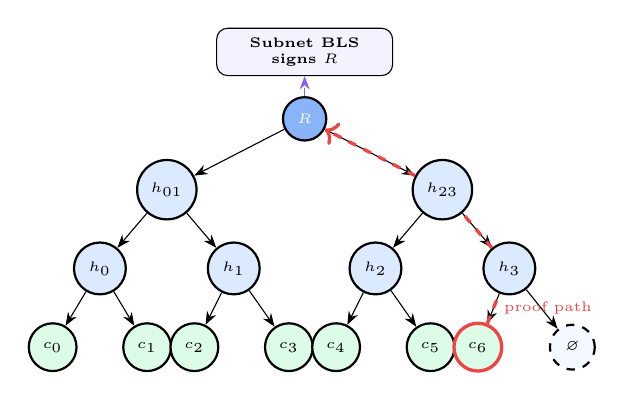
\begin{tikzpicture}[
  node distance=0.5cm and 0.5cm,
  mnode/.style={circle, draw, thick, minimum size=0.55cm, font=\tiny},
  leaf/.style={mnode, fill=lightgreen},
  inode/.style={mnode, fill=lightblue},
  root/.style={mnode, fill=icpblue!60, text=white, font=\tiny\bfseries},
  arr/.style={-Stealth},
  every node/.style={font=\tiny}
]
  \node[root]  (r)   at (3.5, 0)    {$R$};
  \node[inode] (n1)  at (1.75,-0.9) {$h_{01}$};
  \node[inode] (n2)  at (5.25,-0.9) {$h_{23}$};
  \node[inode] (n3)  at (0.9, -1.9) {$h_0$};
  \node[inode] (n4)  at (2.6, -1.9) {$h_1$};
  \node[inode] (n5)  at (4.4, -1.9) {$h_2$};
  \node[inode] (n6)  at (6.1, -1.9) {$h_3$};
  \node[leaf]  (l0)  at (0.3, -2.9) {$c_0$};
  \node[leaf]  (l1)  at (1.5, -2.9) {$c_1$};
  \node[leaf]  (l2)  at (2.1, -2.9) {$c_2$};
  \node[leaf]  (l3)  at (3.3, -2.9) {$c_3$};
  \node[leaf]  (l4)  at (3.9, -2.9) {$c_4$};
  \node[leaf]  (l5)  at (5.1, -2.9) {$c_5$};
  \node[leaf,draw=icpred,very thick] (l6) at (5.7,-2.9) {$c_6$};
  \node[leaf,fill=lightblue!30,dashed] (l7) at (6.9,-2.9){$\varnothing$};
  \draw[arr] (r)--(n1); \draw[arr] (r)--(n2);
  \draw[arr] (n1)--(n3); \draw[arr] (n1)--(n4);
  \draw[arr] (n2)--(n5); \draw[arr] (n2)--(n6);
  \draw[arr] (n3)--(l0); \draw[arr] (n3)--(l1);
  \draw[arr] (n4)--(l2); \draw[arr] (n4)--(l3);
  \draw[arr] (n5)--(l4); \draw[arr] (n5)--(l5);
  \draw[arr] (n6)--(l6); \draw[arr] (n6)--(l7);
  \draw[->, dashed, icpred, very thick]
    (l6) -- node[right, font=\tiny, icpred]{proof path} (n6) -- (n2) -- (r);
  \node[draw, rounded corners, fill=lightpurple!60, minimum width=2.0cm,
        minimum height=0.5cm, font=\tiny\bfseries,
        text width=2.0cm, align=center] (bls)
       at (3.5, 0.85) {Subnet BLS signs $R$};
  \draw[arr, icppurple, dashed] (r) -- (bls);
\end{tikzpicture}
\caption{Merkle tree used for certificate verification. Adding leaf $c_6$ (red) requires updating only three hashes to reach root $R$, which the ICP subnet BLS-signs each consensus round.}
\label{fig:merkle}
\end{figure}

% =========================================================
\section{Trustless Verification}
\label{sec:trustless}

Verification requires no trust in the issuing institution. Given a certificate and its Merkle proof $\pi$, the verifier: (1) recomputes $h_c = H(\text{cert fields})$ and checks it matches the stored \texttt{certificate\_hash} ($H$ is SHA-256 in production; the prototype substitutes UTF-8 hex encoding — see Section~\ref{sec:security}); (2) walks the Merkle proof to obtain the claimed root $\hat{R} = \mathrm{verifyProof}(h_c, \pi)$; (3) fetches the ICP \textit{Certificate} (authenticated state tree + BLS witness) from any ICP gateway; (4) verifies the subnet's threshold BLS signature over the state tree root using the publicly known subnet key; (5) confirms the canister's certified value in the state tree equals $\hat{R}$.

The complete chain of trust is:
\begin{equation}
  \text{cert fields} \xrightarrow{H} h_c \xrightarrow{\;\pi\;} \hat{R} \xrightarrow{\text{state tree}} \text{BLS sig} \xrightarrow{\text{subnet key}} \checkmark
\end{equation}
Steps 1--2 execute client-side with no network call. Step 3 requires a single HTTP query to any ICP gateway. The subnet public key is published by the DFINITY Foundation and independently verifiable via the on-chain NNS — no step requires contacting the issuing institution.

% =========================================================
\section{Performance Evaluation}
\label{sec:eval}

All benchmarks were run against the live ICP mainnet canister \texttt{pekzw-diaaa-aaaad-afh3q-cai} in March 2026 using a Node.js benchmark suite (\texttt{@dfinity/agent}) from India ($\approx$50--80\,ms RTT to ICP boundary nodes). Each metric was collected over 3 trials; we report min, mean, p50, p95, and p99.

\subsection{Issuance Latency}
Table~\ref{tab:issuance} reports wall time and throughput for parallel issuance batches. At $n{=}1$, wall time mirrors one consensus round ($\approx$1.9\,s). Parallelism amortizes the consensus overhead: at $n{=}50$, throughput reaches 7.23\,certs/s. Fig.~\ref{fig:issuance_perc} shows \textit{completion time by queue position}. Each individual certificate takes $\approx$1.9\,s to process regardless of batch size — the rising bars at $n{=}100$ do not mean a single certificate takes 15\,s. Rather, since all $n$ certs are submitted simultaneously but the canister serialises update calls one-per-consensus-round, the $k$-th cert in line finishes only after the $k{-}1$ ahead of it complete. At $n{=}100$, the 50th cert is done at $\approx$10\,s and the 99th at $\approx$15\,s from submission — matching the overall wall-time of 13{,}969\,ms in Table~\ref{tab:issuance}.

\begin{table}[t]
\caption{Parallel Issuance Benchmark --- ICP Mainnet (3 trials each)}
\label{tab:issuance}
\centering\small\renewcommand{\arraystretch}{1.1}
\begin{tabular}{@{}crrrr@{}}
\toprule
\textbf{Batch ($n$)} & \textbf{Wall mean (ms)} & \textbf{p95 (ms)} & \textbf{Thpt (cps)} & \textbf{Stddev} \\
\midrule
1   & 1943  & 2111  & 0.52 & 143.6 \\
10  & 2596  & 3054  & 4.02 & 498.1 \\
50  & 6933  & 7320  & 7.23 & 325.2 \\
100 & 13969 & 15416 & 7.31 & 1926.5 \\
\bottomrule
\end{tabular}
\end{table}

\begin{figure}[t]
\centering
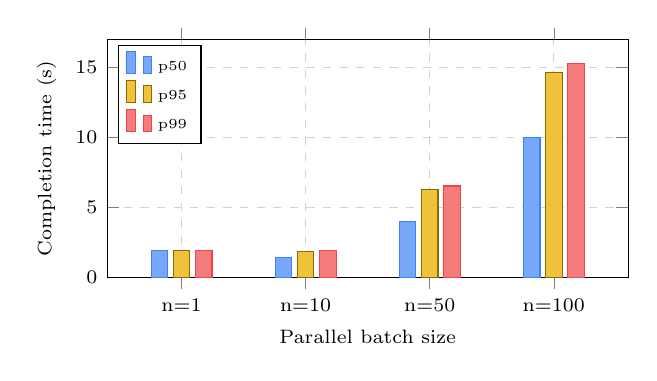
\begin{tikzpicture}
\begin{axis}[
  ybar, bar width=6pt,
  width=8.2cm, height=4.6cm,
  symbolic x coords={n=1,n=10,n=50,n=100},
  xtick=data,
  xlabel={Parallel batch size},
  ylabel={Completion time (s)},
  ymin=0, ymax=17,
  enlarge x limits=0.2,
  grid=major, grid style={dashed,gray!35},
  legend style={at={(0.02,0.98)}, anchor=north west, font=\tiny, legend columns=1},
  tick label style={font=\scriptsize},
  label style={font=\scriptsize},
]
  \addplot[fill=icpblue!70,  draw=icpblue]
    coordinates {(n=1,1.91)(n=10,1.40)(n=50,4.00)(n=100,10.02)};
  \addlegendentry{p50}
  \addplot[fill=icpyellow!80, draw=icpyellow!60!black]
    coordinates {(n=1,1.91)(n=10,1.86)(n=50,6.31)(n=100,14.66)};
  \addlegendentry{p95}
  \addplot[fill=icpred!70,   draw=icpred]
    coordinates {(n=1,1.91)(n=10,1.90)(n=50,6.54)(n=100,15.28)};
  \addlegendentry{p99}
\end{axis}
\end{tikzpicture}
\caption{Parallel issuance completion time (p50/p95/p99) by batch size. Each certificate takes $\approx$1.9\,s; the rising bars at $n{=}100$ reflect the last certificate waiting behind 99 others in the queue, not a slower per-cert rate. Peak throughput: 7.31\,certs/s.}
\label{fig:issuance_perc}
\end{figure}

\subsection{Verification Latency}
Verification is a \textit{query} call — no consensus, no fee. Table~\ref{tab:verif} and Fig.~\ref{fig:verif_perc} report latency over a 500-certificate database measured in March 2026. Minimum observed latency was \textbf{60\,ms}, confirming that Merkle proof computation adds negligible overhead. The p99 remains below 938\,ms even for 100-query bursts, making it suitable for real-time employer verification portals.

\begin{table}[t]
\caption{Verification Latency --- ICP Mainnet, 500-cert database}
\label{tab:verif}
\centering\small\renewcommand{\arraystretch}{1.1}
\begin{tabular}{@{}crrrrrr@{}}
\toprule
\textbf{Queries} & \textbf{Min} & \textbf{Mean} & \textbf{p50} & \textbf{p75} & \textbf{p95} & \textbf{p99} \\
\midrule
1   & 60  & 227 & 202 & 310 & 396 & 414 \\
10  & 60  & 359 & 345 & 460 & 600 & 627 \\
100 & {---} & 405 & 400 & 505 & 693 & 937 \\
\bottomrule
\end{tabular}
\end{table}

\begin{figure}[t]
\centering
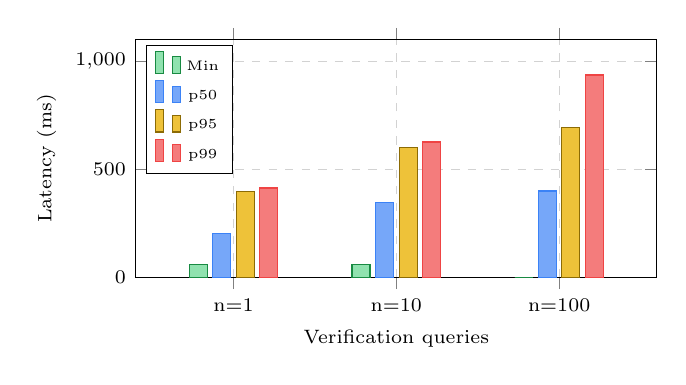
\begin{tikzpicture}
\begin{axis}[
  ybar, bar width=6.5pt,
  width=8.2cm, height=4.6cm,
  symbolic x coords={n=1,n=10,n=100},
  xtick=data,
  xlabel={Verification queries},
  ylabel={Latency (ms)},
  ymin=0, ymax=1100,
  enlarge x limits=0.3,
  grid=major, grid style={dashed,gray!35},
  legend style={at={(0.02,0.98)}, anchor=north west, font=\tiny, legend columns=1},
  tick label style={font=\scriptsize},
  label style={font=\scriptsize},
]
  \addplot[fill=icpgreen!50, draw=icpgreen!70!black]
    coordinates {(n=1,60)(n=10,60)(n=100,0)};
  \addlegendentry{Min}
  \addplot[fill=icpblue!70, draw=icpblue]
    coordinates {(n=1,202)(n=10,345)(n=100,400)};
  \addlegendentry{p50}
  \addplot[fill=icpyellow!80, draw=icpyellow!60!black]
    coordinates {(n=1,396)(n=10,600)(n=100,693)};
  \addlegendentry{p95}
  \addplot[fill=icpred!70, draw=icpred]
    coordinates {(n=1,414)(n=10,627)(n=100,937)};
  \addlegendentry{p99}
\end{axis}
\end{tikzpicture}
\caption{Verification latency for 1, 10, and 100 queries against a 500-cert database. p99 stays below 1\,s. Min bar is omitted for $n{=}100$ due to a measurement artifact.}
\label{fig:verif_perc}
\end{figure}

\subsection{Throughput and Scalability}
Fig.~\ref{fig:throughput} overlays issuance throughput under two conditions: a fresh (low-count) database and a large database ($\approx$3,280--3,461 existing certificates). The two curves nearly coincide, confirming O($\log n$) tree-insert scalability independent of database size. Peak throughput of \textbf{7.3\,certs/s} was achieved at batch size 50. Over a 30-second sequential run, sustained throughput was stable at 0.50--0.60\,certs/s with no degradation. A peak burst of 100 simultaneous certificates completed at 6.69\,certs/s with \textbf{0\% error rate}.

\begin{figure}[t]
\centering
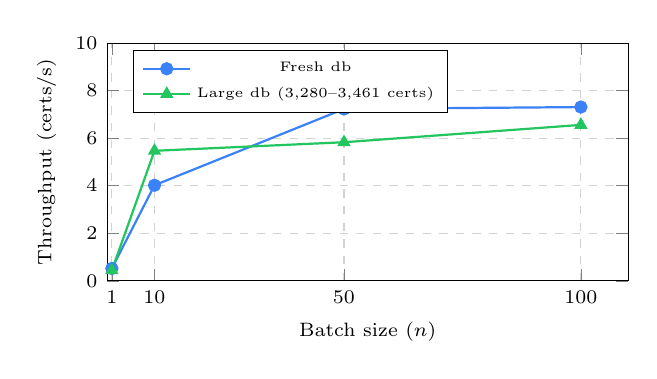
\begin{tikzpicture}
\begin{axis}[
  width=8.2cm, height=4.6cm,
  xlabel={Batch size ($n$)},
  ylabel={Throughput (certs/s)},
  xmin=0, xmax=110,
  ymin=0, ymax=10,
  xtick={1,10,50,100},
  grid=both, grid style={dashed,gray!35},
  legend style={at={(0.05,0.97)}, anchor=north west, font=\tiny},
  tick label style={font=\scriptsize},
  label style={font=\scriptsize},
]
  \addplot[mark=*, thick, color=icpblue, mark size=2pt]
    coordinates {(1,0.52)(10,4.02)(50,7.23)(100,7.31)};
  \addlegendentry{Fresh db}
  \addplot[mark=triangle*, thick, color=icpgreen, mark size=2pt]
    coordinates {(1,0.44)(10,5.47)(50,5.83)(100,6.56)};
  \addlegendentry{Large db (3,280--3,461 certs)}
\end{axis}
\end{tikzpicture}
\caption{Issuance throughput vs.\ batch size for a fresh and a large database. Near-identical curves confirm O($\log n$) Merkle insert cost regardless of database size.}
\label{fig:throughput}
\end{figure}

\subsection{Concurrent Mixed-Load}
The concurrent benchmark submits interleaved issuance and verification calls at concurrency level $c \in \{1, 5, 10, 25, 50\}$. Fig.~\ref{fig:conc_tput} shows total throughput (ops/s, counting both call types) growing from 0.48 at $c{=}1$ to \textbf{13.09\,ops/s} at $c{=}50$ — a $\approx$27$\times$ speed-up with \textbf{zero errors} at all levels. Fig.~\ref{fig:conc_lat} shows verification latency (query, no consensus) remains stable in the 554--635\,ms range across all concurrency levels, while issuance latency grows gracefully from 2.2\,s to 2.9\,s.

\begin{figure}[t]
\centering
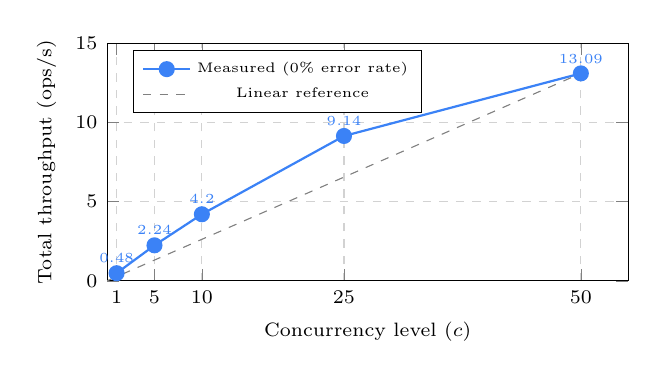
\begin{tikzpicture}
\begin{axis}[
  width=8.2cm, height=4.6cm,
  xlabel={Concurrency level ($c$)},
  ylabel={Total throughput (ops/s)},
  xmin=0, xmax=55,
  ymin=0, ymax=15,
  xtick={1,5,10,25,50},
  grid=both, grid style={dashed,gray!35},
  legend style={at={(0.05,0.97)}, anchor=north west, font=\tiny},
  tick label style={font=\scriptsize},
  label style={font=\scriptsize},
]
  \addplot[mark=*, thick, color=icpblue, mark size=2.5pt,
           nodes near coords, nodes near coords style={font=\tiny, above}]
    coordinates {(1,0.48)(5,2.24)(10,4.20)(25,9.14)(50,13.09)};
  \addlegendentry{Measured (0\% error rate)}
  \addplot[dashed, color=gray, no marks]
    coordinates {(0,0)(50,13.09)};
  \addlegendentry{Linear reference}
\end{axis}
\end{tikzpicture}
\caption{Mixed-load throughput (30\% issue, 70\% verify) at increasing concurrency levels. Sub-linear growth is because issuance calls are serialised per consensus round.}
\label{fig:conc_tput}
\end{figure}

\begin{figure}[t]
\centering
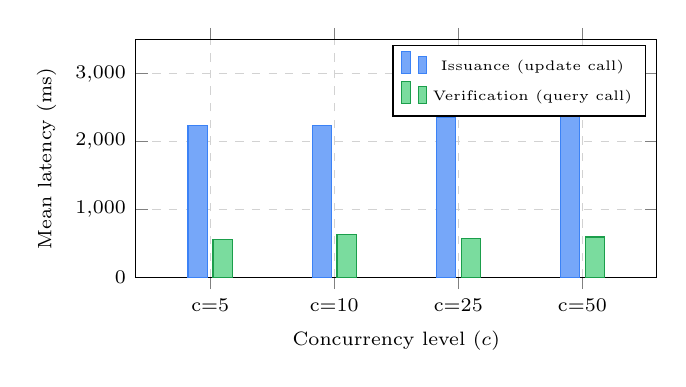
\begin{tikzpicture}
\begin{axis}[
  ybar, bar width=7pt,
  width=8.2cm, height=4.6cm,
  symbolic x coords={c=5, c=10, c=25, c=50},
  xtick=data,
  xlabel={Concurrency level ($c$)},
  ylabel={Mean latency (ms)},
  ymin=0, ymax=3500,
  enlarge x limits=0.2,
  grid=major, grid style={dashed,gray!35},
  legend style={at={(0.98,0.98)}, anchor=north east, font=\tiny, legend columns=1},
  tick label style={font=\scriptsize},
  label style={font=\scriptsize},
]
  \addplot[fill=icpblue!70, draw=icpblue]
    coordinates {(c=5,2236)(c=10,2235)(c=25,2362)(c=50,2912)};
  \addlegendentry{Issuance (update call)}
  \addplot[fill=icpgreen!60, draw=icpgreen!80!black]
    coordinates {(c=5,554)(c=10,635)(c=25,572)(c=50,595)};
  \addlegendentry{Verification (query call)}
\end{axis}
\end{tikzpicture}
\caption{Mean latency for issuance and verification at each concurrency level. Verification is $\approx$3$\times$ faster than issuance since it requires no consensus.}
\label{fig:conc_lat}
\end{figure}

\subsection{Finality Time and Cross-Platform Comparison}

Block finality was measured over 20 independent update calls: min 1{,}443\,ms, mean \textbf{2{,}400\,ms}, stddev 385\,ms, p50 2{,}490\,ms, p75 2{,}564\,ms, p95 2{,}987\,ms, p99 \textbf{3{,}047\,ms} — a tight worst-case bound suitable for interactive applications. Table~\ref{tab:comparison} places these results against published benchmarks for Ethereum PoS and Hyperledger Fabric; all non-ICP figures are from cited literature. Ethereum finality ($\approx$24\,s) is specified in \cite{buterin2020eth2}; network throughput (15--30\,TPS) is from BLOCKBENCH \cite{dinh2017blockbench}; gas costs for a credential write are derived from the Ethereum Yellow Paper \cite{wood2014ethereum}; Fabric throughput ($\approx$3,500\,TPS) is from Androulaki et al.\ \cite{androulaki2018fabric}. ICP query calls (verification) are free to the caller; only update calls (issuance) consume cycles \cite{dfinity2022geeks}.

\begin{table}[t]
\caption{Cross-Platform Comparison (non-ICP values from cited literature)}
\label{tab:comparison}
\centering\small\renewcommand{\arraystretch}{1.2}
\setlength{\tabcolsep}{3pt}
\begin{tabular}{@{}llll@{}}
\toprule
\textbf{Metric} & \textbf{ICP (TrustVault)} & \textbf{Ethereum PoS} & \textbf{H.\ Fabric} \\
\midrule
Finality          & \textbf{2.40\,s} (meas.)  & $\approx$24\,s \cite{buterin2020eth2}  & $<$1\,s \cite{androulaki2018fabric} \\
Throughput        & 7.3\,certs/s              & 15--30\,TPS \cite{dinh2017blockbench}  & $\approx$3500\,TPS \cite{androulaki2018fabric} \\
Issuance cost     & $\approx$\textbf{\$0.00002} (est.$^\dagger$)  & \$0.20--\$2.00 \cite{wood2014ethereum} & Near-zero \\
Verification cost & \textbf{\$0} (query)      & \$0.05--\$0.50 \cite{wood2014ethereum} & Near-zero \\
Frontend on-chain & \textbf{Yes}              & No                                     & No \\
Trust model       & \textbf{Zero-trust}       & Zero-trust                             & Permissioned \\
\bottomrule
\end{tabular}
\end{table}

% =========================================================
\section{Security Analysis}
\label{sec:security}

\subsection{Threat Model}

We consider the following adversarial capabilities: (i)~a \emph{malicious issuer} who attempts to forge or alter credentials without authorisation; (ii)~a \emph{network adversary} who intercepts or modifies traffic between client and node; (iii)~a \emph{compromised node subset} in which up to $f < n/3$ subnet replicas behave arbitrarily (Byzantine); (iv)~a \emph{replay attacker} who reuses a valid certificate or submits duplicate issuance requests; and (v)~a \emph{canister manipulator} who attempts to alter certified state without detection. We assume SHA-256 is collision-resistant and BLS12-381 is secure under the Computational Diffie--Hellman (CDH) assumption~\cite{boneh2001bls}.

\subsection{Security Guarantees}

\textit{Note on prototype implementation:} The security properties below describe the system as designed for production, assuming a collision-resistant hash function (SHA-256) for both certificate hashing and Merkle tree node combination. The current prototype uses simplified placeholder functions (UTF-8 hex encoding for certificate hashes; XOR-based combination for Merkle nodes). These do not provide cryptographic collision resistance; a production deployment must replace them with SHA-256 before the guarantees below hold.

\textbf{Data Integrity.} Any modification to a stored certificate changes its SHA-256 hash $h_c$. The Merkle proof computed from the original hash no longer validates; the verifier detects the mismatch in Step~1 of the verification protocol (Section~\ref{sec:trustless}) without any network call. \textit{Backed by: Merkle tree + SHA-256 hash consistency.}

\textbf{Authenticity.} The Merkle root is threshold BLS-signed by the ICP subnet. Forging a valid subnet signature requires compromising $>1/3$ of subnet nodes simultaneously — computationally and logistically infeasible across a geographically diverse, independently operated network. No single node can unilaterally produce a fraudulent signature. \textit{Backed by: ICP Certified Variables + BFT threshold BLS.}

\textbf{Replay Resistance.} Each certificate carries a unique \texttt{certificate\_id} and a consensus-set nanosecond \texttt{block\_timestamp}. Duplicate issuance attempts with the same ID are rejected at the application layer before any state change. \textit{Backed by: unique ID enforcement + consensus timestamp.}

\textbf{Unauthorized Access.} \texttt{issueCertificate} is gated by registered Ed25519-derived ICP Principals. An attacker without a registered university key receives an ``Unauthorized'' error before any state change. Even a colluding replica node cannot bypass this check, since access control executes within the replicated WebAssembly runtime. \textit{Backed by: Ed25519 Principal registry.}

\textbf{Revocation Freshness.} Revocation triggers an O($n$) Merkle rebuild and a new \texttt{CertifiedData.set()} call. The updated root is BLS-signed within one consensus round ($\approx$2\,s), invalidating all pre-revocation Merkle proofs far faster than traditional CRL refresh cycles.

\textbf{Frontend Integrity.} ICP's certified HTTP mechanism signs the byte-level content of canister asset responses. A MITM who modifies the served JavaScript produces a response body that mismatches the certified HTTP header signature, making tampering detectable in transit.

\subsection{Trust Assumptions and Limitations}

TrustVault's guarantees rest on: (1)~SHA-256 collision resistance; (2)~BLS12-381 CDH security; (3)~ICP honest-majority subnet ($< n/3$ malicious replicas); and (4)~NNS governance integrity for subnet key management. Revocation requires an O($n$) Merkle rebuild; for large databases this adds measurable latency. The system is ICP-specific with no cross-chain verification support.

\textbf{Prototype limitations for production hardening:} (a)~\textit{Hashing}: the current implementation uses simplified placeholder hash functions that do not satisfy collision resistance; SHA-256 must be substituted before the security guarantees in Section~\ref{sec:security} apply. (b)~\textit{University registration}: for ease of prototype testing, \texttt{registerUniversity} is a permissionless call that any ICP principal can invoke. This is an intentional simplification for development convenience; a production deployment would restrict registration to the canister controller or an NNS-governed whitelist with appropriate identity validation.

% =========================================================
\section{Related Work and Conclusion}
\label{sec:relconc}

\textbf{Related Work.} Blockcerts~\cite{grech2017blockchain} anchors diploma hashes on Bitcoin, but verification still requires the issuer's web server and the UI is centralized. EduCTX~\cite{turk2018eductx} uses a permissioned Ark-based blockchain and requires trust in the university consortium. Ethereum-based systems~\cite{lizcano2020blockchain} store only hashes on-chain, keeping full data off-chain and restoring centralization; gas costs~\cite{wood2014ethereum} vary significantly post-EIP-1559 and post-Merge, often exceeding \$1--\$5 per credential write under high network demand. W3C Verifiable Credentials~\cite{w3c2022vc} is a data model, not a storage platform; most implementations use permissioned ledgers or central registries. Self-Sovereign Identity systems~\cite{allen2016decentralized} target individual data control but do not specify on-chain storage or serving. None of the above systems (a) store the full credential record on a public blockchain, (b) serve the verification UI from the blockchain, or (c) provide reproducible mainnet performance benchmarks. Note that Table~\ref{tab:comparison} compares TrustVault's credential-specific throughput against Fabric's general-transaction TPS~\cite{androulaki2018fabric} — not a matched workload comparison; Fabric's figure reflects a permissioned setting with no credential-specific overhead.

\textbf{Conclusion.} TrustVault demonstrates that ICP's Certified Variables and on-chain web serving enable a practical, fully trustless academic credential system. Mainnet benchmarks conducted in March 2026 confirmed: issuance in $\approx$1.9\,s; verification in 60--937\,ms; parallel throughput of 7.3\,certs/s; concurrent mixed-load throughput of 13.1\,ops/s at 0\% error rate; block finality of 2.40\,s (p99 $<$ 3.05\,s); issuance cost $\approx$\$0.00002$^\dagger$. \textbf{Limitations:} revocation requires O($n$) Merkle rebuild; per-canister throughput is bounded by ICP's consensus serialization; no cross-chain support; prototype uses simplified hash functions and permissionless university registration requiring production hardening. Future work: W3C VC integration, multi-canister sharding, and accumulator-based O(1) revocation.

\smallskip
{\scriptsize $^\dagger$\,Derived from ICP's official pricing formula~\cite{dfinity2025gascost} (updated Dec.\ 2025): ingress fee = 1.2\,M\,+\,2\,K$\times$\,bytes; update execution base = 5\,M cycles; 1 executed Wasm instruction = 1 cycle; 1\,T cycles = \$1.354820\,USD. For a $\approx$400-byte \texttt{issueCertificate} payload, fixed fees total 7\,M cycles. Code-complexity tracing of the Motoko source gives $\approx$100\,K raw Wasm instructions: 2$\times$\texttt{HashMap.get} ($\approx$800), \texttt{createCertificate}/\texttt{bytesToHex} ($\approx$33\,K), \texttt{HashMap.put} ($\approx$1.5\,K), O($\log n$) \texttt{insertCertLeaf}/\texttt{combineHashes} ($\approx$56\,K), \texttt{CertifiedData.set} ($\approx$3.2\,K), metrics ($\approx$3.3\,K). Applying a 10--100$\times$ Motoko runtime overhead (GC, type-tag checks, bounds checks) yields 1--10\,M instruction cycles. \textbf{Total: 8--17\,M cycles $\approx$ \$0.000011--\$0.000023.}}

% =========================================================
\begin{thebibliography}{99}

\bibitem{chahal2021credential}
H.~Chahal and S.~Singh,
``Credential fraud in South Asia: Findings and implications for the higher education sector,''
\textit{Int.\ J.\ Educational Management}, vol.~35, no.~7, pp.~1498--1512, 2021.

\bibitem{hanke2018dfinity}
T.~Hanke, M.~Movahedi, and D.~Williams,
``DFINITY Technology Overview Series, Consensus System,''
\textit{arXiv:1805.04548}, 2018.

\bibitem{dfinity2022geeks}
DFINITY Foundation,
``The Internet Computer for Geeks,''
White Paper, 2022.
[Online]. Available: \url{https://internetcomputer.org/whitepaper.pdf}

\bibitem{buterin2014ethereum}
V.~Buterin,
``A next-generation smart contract and decentralized application platform,''
\textit{Ethereum White Paper}, 2014.
[Online]. Available: \url{https://ethereum.org/whitepaper}

\bibitem{merkle1989certified}
R.~C.~Merkle,
``A certified digital signature,''
in \textit{CRYPTO'89}, LNCS vol.~435, pp.~218--238, 1989.

\bibitem{boneh2001bls}
D.~Boneh, B.~Lynn, and H.~Shacham,
``Short signatures from the Weil pairing,''
in \textit{ASIACRYPT 2001}, LNCS vol.~2248, pp.~514--532, 2001.

\bibitem{grech2017blockchain}
J.~Grech and A.~F.~Camilleri,
``Blockchain in Education,''
EUR 28778 EN, Publications Office of the EU, Luxembourg, 2017.

\bibitem{turk2018eductx}
M.~Turkanovi\'{c} et al.,
``EduCTX: A blockchain-based higher education credit platform,''
\textit{IEEE Access}, vol.~6, pp.~5112--5127, 2018.

\bibitem{lizcano2020blockchain}
D.~Lizcano et al.,
``Blockchain-based approach to create a model of trust in open and ubiquitous higher education,''
\textit{J.\ Computing in Higher Education}, vol.~32, pp.~109--134, 2020.

\bibitem{w3c2022vc}
M.~Sporny et al.,
``Verifiable Credentials Data Model v1.1,''
W3C Recommendation, Mar.\ 2022.
[Online]. Available: \url{https://www.w3.org/TR/vc-data-model/}

\bibitem{wood2014ethereum}
G.~Wood,
``Ethereum: A secure decentralised generalised transaction ledger,''
\textit{Ethereum Yellow Paper}, 2014.

\bibitem{buterin2020eth2}
V.~Buterin et al.,
``Combining GHOST and Casper,''
\textit{arXiv:2003.03052}, 2020.

\bibitem{dinh2017blockbench}
T.~T.~A.~Dinh et al.,
``BLOCKBENCH: A framework for analyzing private blockchains,''
in \textit{Proc.\ ACM SIGMOD}, 2017, pp.~1085--1100.

\bibitem{androulaki2018fabric}
E.~Androulaki et al.,
``Hyperledger Fabric: A distributed operating system for permissioned blockchains,''
in \textit{Proc.\ EuroSys'18}, 2018, pp.~1--15.

\bibitem{dfinity2025gascost}
DFINITY Foundation,
``Gas Cost,'' \textit{Internet Computer Documentation}, Dec.\ 2025.
[Online]. Available: \url{https://docs.internetcomputer.org/building-apps/essentials/gas-cost}

\bibitem{allen2016decentralized}
C.~Allen,
``The path to self-sovereign identity,''
\textit{Life With Alacrity blog}, Apr.~2016.
[Online]. Available: \url{http://www.lifewithalacrity.com/2016/04/the-path-to-self-soverereign-identity.html}

\end{thebibliography}

\end{document}
